%!TEX root = ../thesis.tex
%*******************************************************************************
%*********************************** First Chapter *****************************
%*******************************************************************************

\chapter{Introduction}  %Title of the First Chapter

\ifpdf
    \graphicspath{{Chapter1/Figs/Raster/}{Chapter1/Figs/PDF/}{Chapter1/Figs/}}
\else
    \graphicspath{{Chapter1/Figs/Vector/}{Chapter1/Figs/}}
\fi


%**********************************

%********************************** %First Section  **************************************

\nomenclature[x]{$F$}{Boolean Formula}
\nomenclature[z-CNF]{CNF}{Conjunctive Normal Form}
\nomenclature[z-DNF]{DNF}{Disjunctive Normal Form}
\nomenclature[z-SAT]{SAT}{Boolean Satisfiability Problem}
\nomenclature[z-kSAT]{$k$-SAT}{Boolean Satisfiability Problem with each clause
                               restricted to have size $k$ or less}

\begin{figure}
    \centering
    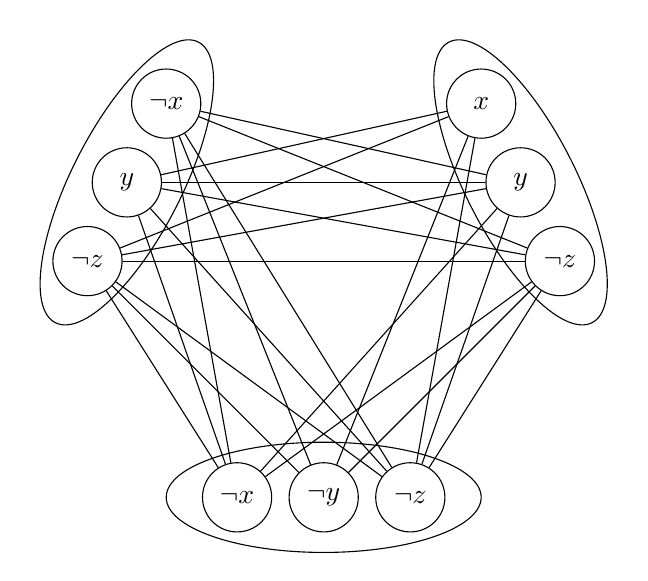
\begin{tikzpicture}
        \begin{scope}[auto,every node/.style={draw,circle,minimum size=2.5em}]
            % Clause 1
            \node (c1!x) at (-2, 0) {$\neg x$};
            \node (c1y) at (-2.5, -1) {$y$};
            \node (c1!z) at (-3, -2) {$\neg z$};
            \draw[rotate around={63:(-2.5,-1)}] (-2.5,-1) ellipse (2 and 0.7);

            % Clause 2
            \node (c2x) at (2, 0) {$x$};
            \node (c2y) at (2.5, -1) {$y$};
            \node (c2!z) at (3, -2) {$\neg z$};
            \draw[rotate around={-63:(2.5,-1)}] (2.5,-1) ellipse (2 and 0.7);

            % Clause 2
            \node (c3!x) at (-1.1, -5) {$\neg x$};
            \node (c3!y) at (0, -5) {$\neg y$};
            \node (c3!z) at (1.1, -5) {$\neg z$};
            \draw[] (0,-5) ellipse (2 and 0.7);
        \end{scope}
        
        \path (c1!x) edge (c2y);
        \path (c1!x) edge (c2!z);
        \path (c1!x) edge (c3!x);
        \path (c1!x) edge (c3!y);
        \path (c1!x) edge (c3!z);
        \path (c1y) edge (c2x);
        \path (c1y) edge (c2y);
        \path (c1y) edge (c2!z);
        \path (c1y) edge (c3!x);
        \path (c1y) edge (c3!z);
        \path (c1!z) edge (c2x);
        \path (c1!z) edge (c2y);
        \path (c1!z) edge (c2!z);
        \path (c1!z) edge (c3!x);
        \path (c1!z) edge (c3!y);
        \path (c1!z) edge (c3!z);
        
        \path (c2x) edge (c3!y);
        \path (c2x) edge (c3!z);
        \path (c2y) edge (c3!x);
        \path (c2y) edge (c3!z);
        \path (c2!z) edge (c3!x);
        \path (c2!z) edge (c3!y);
        \path (c2!z) edge (c3!z);
    \end{tikzpicture}
    \caption[Graph Representation of a 3SAT Formula]{Illustration of the 3SAT in Equation \ref{eq:formula_sat}. Vertices are grouped
    by their clauses and the edges
    represent literals that do not contradict. This establishes a reduction
    from 3SAT to clique}
    \label{fig:sat}
\end{figure}

\section{Boolean Satisfiability Problem} %Section - 1.1 
The boolean satisfiability problem, abbreviated as SAT, is the problem of finding
a satisfying assignment to the variables to make a boolean formula evaluate to true.
CNF-SAT is the same problem, but with formulas restricted to Conjunctive Normal Form
(CNF). A boolean formula in CNF is composed of a conjunction of clauses where
each clause is a disjunction of literals. For example consider the following
boolean formula in CNF: 
\begin{equation} \label{eq:formula_sat}
    (\neg x \lor y \lor \neg z) \land (x \lor y \lor \neg z) \land (\neg x \lor \neg y \lor \neg z)
\end{equation}
This boolean formula has
a satisfying assignment $x = \text{false}, y = \text{true}, z = \text{false}$. Therefore the boolean formula is satisfiable.
However, if we consider the boolean formula
\begin{align}
(x \lor y \lor z)\land(x \lor y \lor \neg z)\land(x \lor \neg y \lor z) \nonumber\\
\land(x \lor \neg y \lor \neg z)\land(\neg x \lor y \lor z)\land(\neg x \lor y \lor \neg z) \\
\land(\neg x \lor \neg y \lor z)\land(\neg x \lor \neg y \lor \neg z) \nonumber
\end{align}
It's clear to see that this boolean formula can have no
satisfying assignment, since each assignment to the variables
will at least leave one clause unsatisfied.

%********************************** %Second Section  *************************************
\section{Uses of Boolean Satisfiability} %Section - 1.2
\subsection{Theoretical Significance}
SAT is a widely studied problem and has had a significant impact on
our understanding of computational complexity. For instance, SAT
was the first problem shown to be NP-HARD.
This then forms the basis of the NP-COMPLETE complexity class \cite{cook1971complexity, karp1972reducibility}.
This then means that a large class of problems all can be reduced to each other \cite{garey1974some}.
SAT has then in some sense become the defacto NP-COMPLETE problem and
our understanding of NP-COMPLETEness is driven by our understanding of SAT.

Furthermore, study of SAT has lead to new conjectures about
the complexity of SAT that are stronger than
the $P \neq NP$ conjecture, roughly stating that SAT requires exponential time \cite{impagliazzo2001complexity}. These conjectures allow for new conditional lower
bounds on a wide variety of other problems, not strictly limited to
NP-COMPLETE problems \cite{vassilevska2015hardness, lokshtanov2013lower}.
This gives us an understanding of the relative difficulty of finding
improved algorithms for many computational problems. For instance,
we know that finding a $\mathcal{O}(n^{2 - \epsilon})$ time algorithm
for string edit distance would violate some of these conjectures \cite{vassilevska2015hardness, levenshtein1966binary}. Hence making an improvement over an $\mathcal{O}(n^2)$ algorithm
should be seen as being as hard as discovering an improved SAT algorithm.

\subsection[Practical Applications]{Practical Applications of Boolean Satisfiability}
Although, even with these conjectures about the hardness of SAT,
as SAT solvers have become more efficient, SAT solving has found numerous applications \cite{marques2008practical, sat2009theory}.
One of these applications is model checking, where
the use SAT allows for better memory usage than traditional methods and hence larger models \cite{biere1999symbolic}.
Others include, but are not limited to, crosstalk noise prediction in integrated circuits \cite{chen1999towards},
termination analysis \cite{fuhs2007sat}, design debugging \cite{smith2005fault}, AI planning \cite{kautz1992planning},
haplotype  inference  in  bioinformatics \cite{lynce2006efficient}, knowledge-compilation \cite{darwiche2004new},
software testing \cite{khurshid2004testera}, package management in software distributions \cite{tucker2007opium},
checking of pedigree consistency \cite{10.1007/978-3-540-71209-1_26}, Test-pattern generation in digital systems
\cite{larrabee1992test} and circuit delay computation \cite{mcgeer1991timing}.

Naturally, as the computational power available to SAT solvers grows and as the
solvers become more efficient, SAT solving will find more
practical applications.

%********************************** % Third Section  *************************************
\section{Organisation and Motivation For This Report}  %Section - 1.3 
%NP-COMPLETE decision problems such as SAT and variants such as 3SAT,
%do not have any polynomial time algorithms unless $P=NP$ \cite{schaefer1978complexity}.
%However, SAT is a useful problem in practice \cite{marques2008practical}.
%Therefore, algorithms for solving SAT such as the 
%Davis Putnam Logemann Loveland algorithm (DPLL) and
%Conflict Driven Clause Learning (CDCL) have been developed \cite{Quest_for_efficient_solvers, CDCL}.
%Solvers based on these algorithms appear to be ``fast'' in practice \cite{SAT_Comp2017}.
%At the same time, there are popular conjectures about the complexity
%of SAT that are stronger than assuming $P=NP$ \cite{impagliazzo2001complexity}. These conjectures
%allow theoreticians to prove conditional lower bounds on a wide
%array of problems \cite{lokshtanov2013lower, vassilevska2015hardness}. 
There is a juxtaposition of theory and practice where conjectures about the computational complexity of
SAT suggest that we should not expect it to be solvable in subexponential time \cite{impagliazzo2001complexity},
and yet there are highly optimised SAT solvers that are ``fast'' in practice. Some
of these solvers are able to handle SAT instances having on the order of $10^5$ variables
and $10^6$ clauses \cite{SAT_Comp2017, sat2018descriptions}.
This report will attempt to provide an exposition on this
gap between theory and practice. 

First this will be done by providing an overview of how modern SAT solvers work,
by both covering the algorithms that these solvers are based on and also some
of the implemented solvers that use these algorithms.

To contrast this, the next two chapters will cover the complexity conjectures
that are based on the hardness of SAT and will go over some conditional lower bounds that can be
proven using these conjectures. This report also decides to dedicate a chapter to a commonly used lemma
in these proofs called the sparsification lemma. This lemma is instrumental in many
conditional lower bounds that apply to polynomial time algorithms such as string edit distance, hence
this chapter will explain and go over the proof of the lemma, providing some new intuitions along the way.

Finally, the last chapter will cover some research into structures in SAT instances
that can be used to either explain why some SAT instances are easy to solve compared to what
the worst case complexity of SAT solving would suggest, or provide motivation for currently employed
heuristics in modern SAT solvers.

Taken as a whole this report will provide the reader with a foundational understanding
of both how practical SAT solvers work and how they are able
to solve SAT instances that are significantly larger than what we might expect were possible
given what worst case complexity suggests. This report attempts to be accessible
to anyone with an undergraduate level understanding of computational complexity and algorithms
who is interesting in both the practical and theoretical side of SAT.

%To understand the apparent gap between worst case complexity and practical performance
%a number of empirical studies have been made to illustrate the existence of structure
%within most SAT instances which modern SAT solvers can exploit \cite{DBLP:journals/corr/ZulkoskiMWRLCG17, backdoor_typical, SAT_Comp2017, understanding_sat_structure}.
%Two key realisations
%support the notion that SAT can be solved faster than what worst case complexity would
%suggest. The first being the existence of a ``phase transition'' in the difficulty of instances
%of SAT. That being that as the ratio of clauses to the number of variables in the SAT   
%formula increases, the probability of the SAT formula being satisfiable decreases (as
%there are now more constraints). The apparent ``hardness'' in practice peaks when this
%ratio approaches approximately $0.42$ and SAT instances can be solved significantly quicker
%when the ratio is larger or smaller than $0.42$ \cite{phase_transition, hard_and_easy_distributions}.
%The second discovery, is the existence of strong and weak backdoors in SAT instances \cite{10.1007/978-3-642-21043-3_33, backdoor_typical}.
%A backdoor in a SAT instance is a small subset of literals in the SAT formula such that
%when these literals are satisfied, the remaining subproblem can be solved in polynomial time. Current literature suggest that most SAT instances have backdoors significantly
%smaller than the size of the SAT formula.

\section{Notation}

A brief mention of notation before moving on, unless otherwise specified
a SAT instance will be in Conjunctive Normal Form (CNF), hence
we use the term SAT informally to refer to CNF-SAT. This means that
a formula is a conjunction of clauses where each clause is a disjunction of literals.
In terms of representation, it will often be convenient to represent a clause
$C$ as a set of literals and a formula $F$ as a set of clauses.
Therefore a formula
\begin{equation*}
    F = (a \lor b) \land (\neg a \lor b \lor \neg c) \land (b \lor c)
\end{equation*}
will be represented as
\begin{equation*}
    \{\{a, b\},\{\neg a, b, \neg c\}, \{b, c\}\}
\end{equation*}
Thus we can denote the number of clauses as $|F|$ and we could
express the set of literals as $\bigcup_{C \in F}C$.

Throughout this report, the letters $n$ and $m$ will always denote the
number of variables and the number of clauses respectively. These
parameters of the formula have notable significance on the running time
of algorithms for SAT and variants of SAT. Hence it is often natural
to express the complexity of these algorithms as a parameterized complexity
with often $n$ as the parameter (Although this is not always the case, see \cite{hirsch2000new}).
Often this will give expressions of the
form $2^n \cdot (n + m)^{\mathcal{O}(1)}$. However, the polynomial
factor is not of much interest and hence we will use the notation
$\mathcal{O}^{\ast}(\cdot)$ to suppress any polynomial factors.
$k$-SAT is CNF-SAT with the additional restriction that $\forall C \in F : |C| \leq k$.
For boolean formulas $F$ and $G$, we use the notation $F \approx G$ to mean
that $F$ and $G$ are equisatisfiable.
Let $vars()$ be a function that returns the set of variables that are used
in its argument. So for a formula $F$, then $vars(F)$ is the set of $n$ variables,
for a clause $C$, then $vars(C)$ is the set of variables that appear in the clause
and for a literal $l$, then $vars(l)$ is simply the variable that corresponds to
that literal.